\documentclass[border=10pt]{standalone}
\usepackage[svgnames]{xcolor}
\usepackage{amsmath}
\usepackage{pgfplots}
\pgfplotsset{compat=newest}
\usepackage[sfdefault]{FiraSans}
\usepackage{FiraMono}
\renewcommand*\familydefault{\sfdefault}
\begin{document}
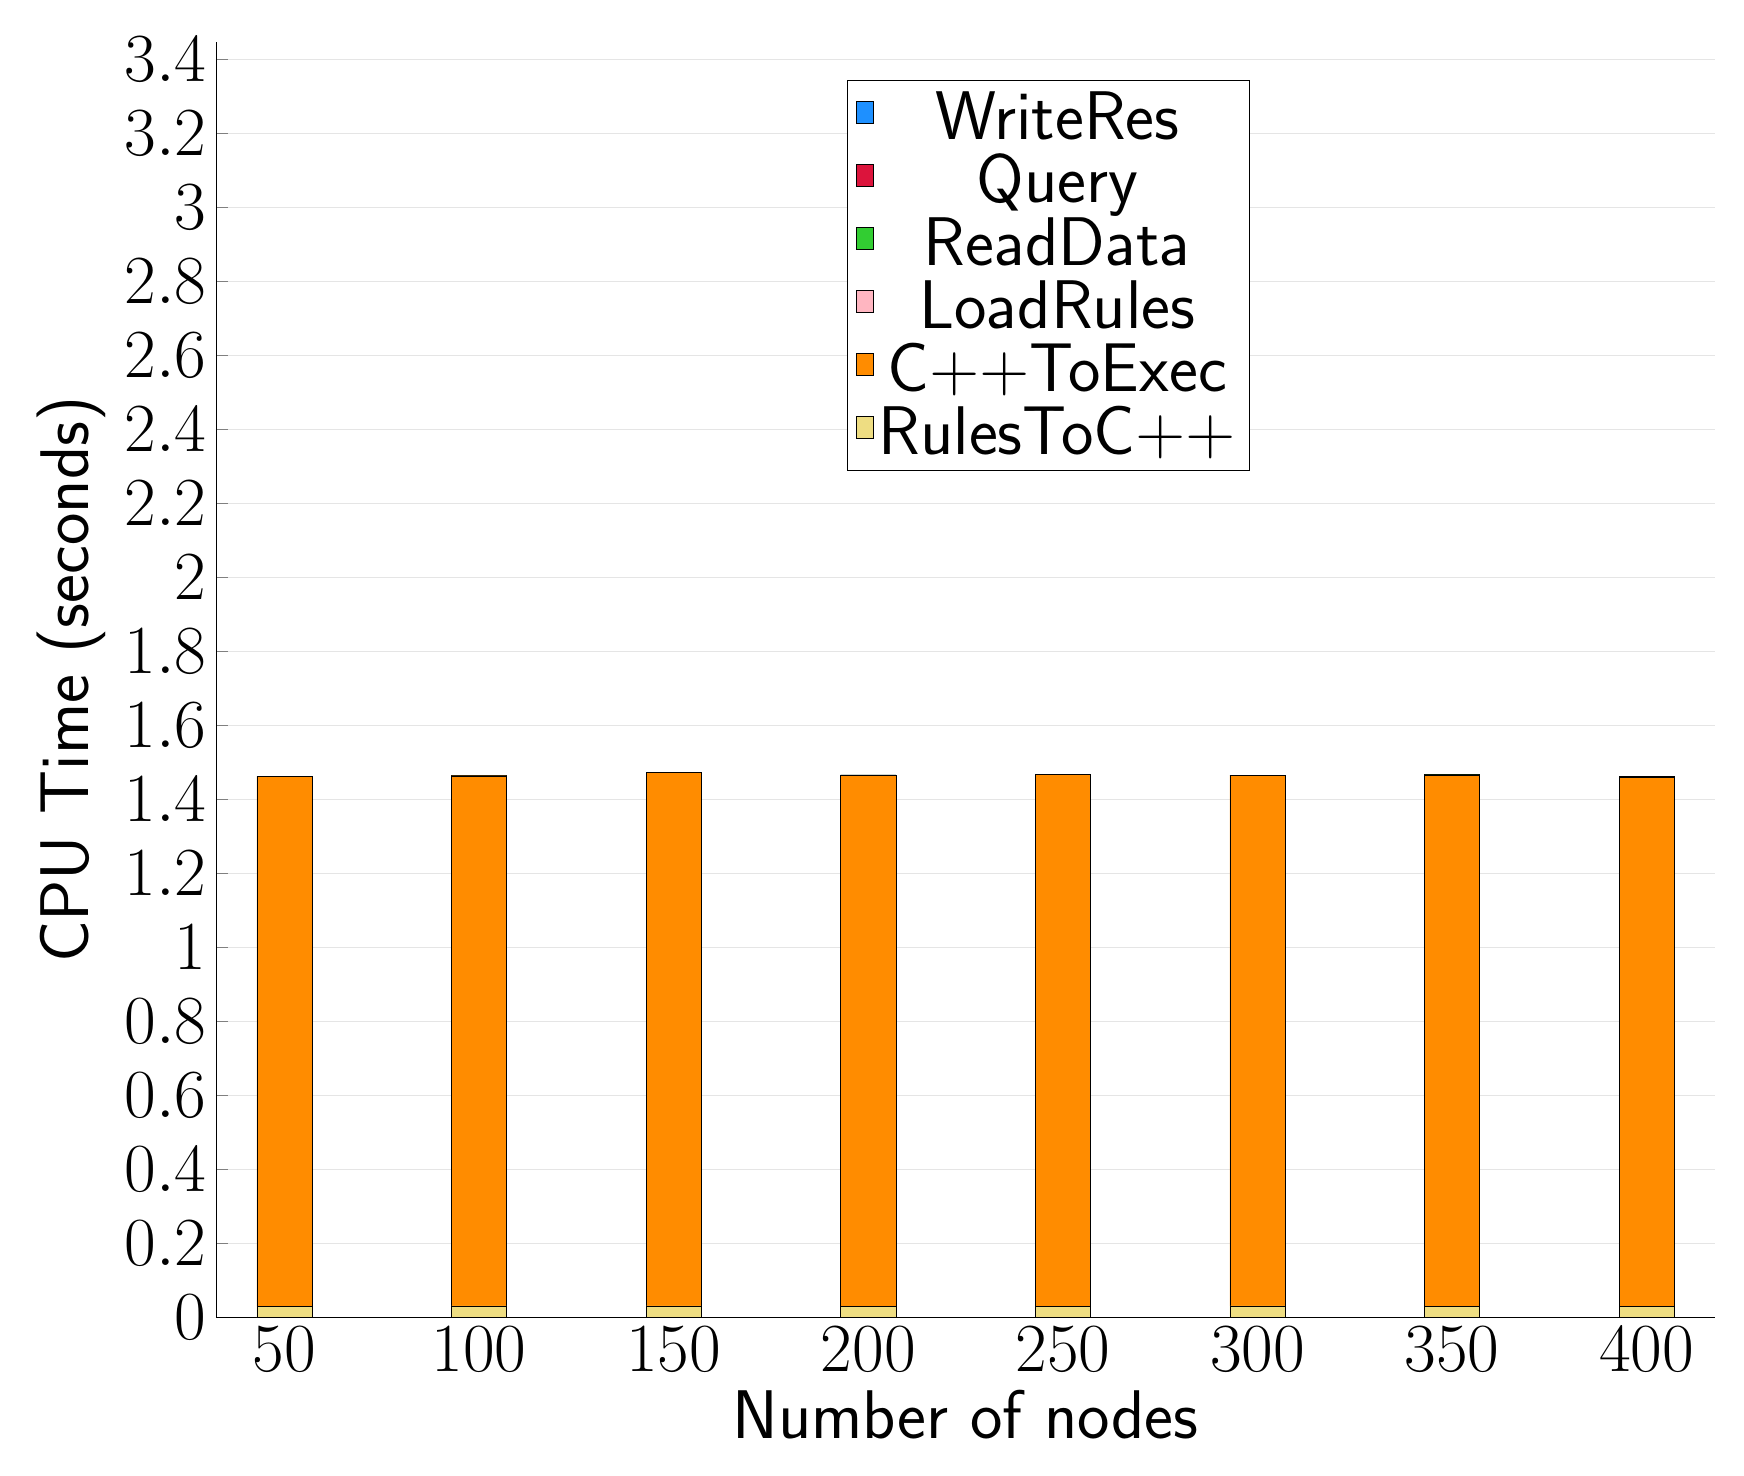
\begin{tikzpicture}
	\begin{axis}[
			ybar stacked,
			width=1.7\textwidth,
			bar width=0.7cm,
			ymajorgrids, tick align=inside,
			major grid style={draw=gray!20},
			xtick=data,
			ymin=0, ymax=3.4459999999999997,
			axis x line*=bottom,
			axis y line*=left,
			enlarge x limits=0.05,
			legend style={
					at={(0.69, 0.97)},
					anchor=north east,
					legend columns=1,
					font=\Huge,
				},
			ylabel={CPU Time (seconds)},
			xlabel={Number of nodes},
			label style={font=\Huge},
			tick label style={font=\Huge},
		]
		\addlegendimage{fill=DodgerBlue, draw=black, line width=0.2pt}
		\addlegendentry{WriteRes}
		\addlegendimage{fill=Crimson, draw=black, line width=0.2pt}
		\addlegendentry{Query}
		\addlegendimage{fill=LimeGreen, draw=black, line width=0.2pt}
		\addlegendentry{ReadData}
		\addlegendimage{fill=LightPink, draw=black, line width=0.2pt}
		\addlegendentry{LoadRules}
		\addlegendimage{fill=DarkOrange, draw=black, line width=0.2pt}
		\addlegendentry{C++ToExec}
		\addlegendimage{fill=LightGoldenrod, draw=black, line width=0.2pt}
		\addlegendentry{RulesToC++}
		\addplot +[fill=LightGoldenrod, draw=black, line width=0.2pt] coordinates {
				(50, 0.030000000000000006)
				(100, 0.031000000000000007)
				(150, 0.031000000000000007)
				(200, 0.030000000000000006)
				(250, 0.030000000000000006)
				(300, 0.031000000000000007)
				(350, 0.030000000000000006)
				(400, 0.030000000000000006)
			};
		\addplot +[fill=DarkOrange, draw=black, line width=0.2pt] coordinates {
				(50, 1.4309999999999998)
				(100, 1.432)
				(150, 1.4409999999999998)
				(200, 1.4349999999999998)
				(250, 1.4369999999999998)
				(300, 1.4329999999999998)
				(350, 1.4349999999999998)
				(400, 1.43)
			};
		\addplot +[fill=LightPink, draw=black, line width=0.2pt] coordinates {
				(50, 0.0)
				(100, 0.0)
				(150, 3.24e-05)
				(200, 1.12e-05)
				(250, 1.1e-05)
				(300, 1.11e-05)
				(350, 0.0)
				(400, 2.19e-05)
			};
		\addplot +[fill=LimeGreen, draw=black, line width=0.2pt] coordinates {
				(50, 0.00038309999999999993)
				(100, 0.00047829999999999997)
				(150, 0.0005902000000000001)
				(200, 0.0007106)
				(250, 0.0007619)
				(300, 0.0009153)
				(350, 0.0009452)
				(400, 0.0011065)
			};
		\addplot +[fill=Crimson, draw=black, line width=0.2pt] coordinates {
				(50, 0.0)
				(100, 5.14e-05)
				(150, 0.0001305)
				(200, 0.00018930000000000002)
				(250, 0.0002215)
				(300, 0.0002798999999999999)
				(350, 0.0003071)
				(400, 0.00035660000000000005)
			};
		\addplot +[fill=DodgerBlue, draw=black, line width=0.2pt] coordinates {
				(50, 0.00021709999999999996)
				(100, 0.0002359)
				(150, 0.0002566)
				(200, 0.0003128)
				(250, 0.00032240000000000003)
				(300, 0.0003357999999999999)
				(350, 0.0003377)
				(400, 0.000361)
			};
	\end{axis}
\end{tikzpicture}

\end{document}
